\chapter{Einführung und Projektidee}
Video über Brühl. Menschen den Brühl näherbringen. Früher belebtes Einkaufsboulevard, nach der Wende verkommen lassen, nun wieder im Aufschwung durch städtisches und privates Engagement. // 360°, VR, 3D, verschiedene tages- und jahreszeiten. in geschäfte und häuser gehen. von oben mit drohne. bestimmte veranstaltungen. vergleich alte fotos // touch, gesten, sprache, bewegung (apparate), maus tastatur // TV, VR, Google Glass (overlay), tablet, pc
\chapter{Design und Konzeption}
Verschiedene Ideen vorstellen -> Anordnung/Aussehen des Players mit Skizze
Warum bestimmte Features nicht umgesetzt / umgesetzt. Einfachheit
\chapter{Ablaufplan}
Videodaten aufzählen mit Details
POI: Brühltor, Schule, Paris, Stuhl, Zuhause, 
\chapter{Implementierung}

Der Player ist in den grundlegenden Webtechniken umgesetzt und da keine serverseitige Technologie wie PHP o.ä. zum Einsatz kommt, ist kein Webserver notwendig.

Anforderungen:
- Internetverbindung
- Kein Webserver notwendig, da komplett mit HTML, CSS und JS umgesetzt

Verwendete Bibliotheken:

- Video.js (Player)

	Open-source HTML5 Video Player
	
- Video.js-Overlay-Plugin (Player Overlays)

	POI-Overlay
	
- Bootstrap (UI Elements)

	Grid-Layout (siehe Bootstrap-Dokumentation, z.B. col-md-4)

- jQuery (common lib for JS)
	
	Easy access and traversing through DOM Tree
	
- XML2JSON

	Convert XML to JSON-Format (https://github.com/sparkbuzz/jQuery-xml2json)
	
Installation:
- Projekt von Github klonen
- Internetverbindung prüfen
- Öffnen des Players über video-bruehl/src/index.html

Information zum XML

---TODO--- steve

\chapter{Zusammenfassung}




\label{kapitel1}
Eine der wohl wichtigsten Säulen unternehmerischer Tätigkeit ist die Interaktion mit Kunden. Sei es im Verkauf, bei der Akquise, in Verhandlungen jeglicher Art oder eben bei der Integration von Kunden in bestimmte Prozesse, sei es im Business-to-Customer- oder im Business-to-Business-Bereich: Unterm Strich bleibt es immer eine Kommunikation von Mensch zu Mensch -- People-to-People.
\\ \\
Da jeder Mensch unterschiedliche Denkmuster aufweist und die gesprochene sowie die Körpersprache des Gegenübers anders interpretiert, kann es bei der Kommunikation zwischen Personen stets zu Verständnisproblemen kommen. Um eine Botschaft, die zunächst in Form von Gefühlen, Wünschen oder einer Meinung existiert, an einen anderen Menschen zu übermitteln, müssen diese Gedanken zu aller erst in menschliche Sprache und/oder Körperbewegungen umgewandelt werden. Über verschiedene Kommunikationskanäle, wie zum Beispiel das gesprochene Wort oder signalisierte Körpersprache, gelangt die codierte Botschaft zum Empfänger. Diese verbale und nonverbale Nachricht muss von ihm nun wieder entschlüsselt und anschließend in Bezug auf die ursprüngliche Intention des Senders hin interpretiert werden. Auf ihrem Weg vom Sender zum Empfänger kann es bei jeder Interpretation oder Umwandlung der Nachricht zu Fehlern kommen, die die ursprüngliche Botschaft verfälschen würde.\footnote{vgl. Hall, 1980, S. 128 ff. \cite{Hall1980}}
\\ \\
Von diesen Schwierigkeiten ist auch die Kommunikation zwischen den Mitarbeitern eines Unternehmens und dessen Kunden betroffen. So können zum Beispiel die Anforderungen und Bedürfnisse von Kunden missverstanden oder von den Kunden selbst falsch übermittelt werden. Andererseits ist es auch möglich, dass ein Unternehmen seine angebotenen Services seinen Zielgruppen falsch und nicht unmissverständlich vermittelt. An diesen problematischen Punkten setzt das GAP-Modell an und zeigt auf, wo diese Differenzen in der Kommunikation zwischen Unternehmen und Kunden lokalisiert sind und wie das gegenseitige Verständnis optimiert werden kann.
\\ \\
In den folgenden Kapiteln werden zunächst die Grundlagen des GAP-Modells und der Kundenintegration erörtert. Darauf folgend werden die Besonderheiten des Modells im Kontext der Kundenintegration im Business-to-Business-Bereich analysiert. Abschließend werden die Erkenntnisse dieser Ausarbeitung zusammengefasst und resümiert, wie diese in der Praxis angewendet werden können.



\chapter{Grundlagen}
\label{kapitel2}
Die folgenden Abschnitte beleuchten die Entstehung des GAP-Modell in Hinblick auf die Dienstleistungsqualität von Unternehmen sowie allgemeine Aspekte der Kundenintegration im Bereich des Business-to-Business-Marketings.
\section{Das GAP-Modell}
Das GAP-Modell wurde in den 80er Jahren von den amerikanischen Wissenschaftlern Valarie A. Zeithaml, Leonard L. Berry und A. Parasuraman als ein Modell für die Servicequalität von Unternehmen im Dienstleistungssektor erarbeitet. Das zur damaligen Zeit vorhandene Wissen über die Beurteilung der Qualität von Waren und Gütern genügte nicht, um gleichfalls Aussagen über die Einschätzung einer Dienstleistungsqualität treffen zu können, da diese deutlich schwerer zu evaluieren ist.\footnote{vgl. Zeithaml/Berry/Parasuraman, 1985, S. 42  \cite{Parasuraman_1985}} Der Entwicklung dieses empirischen Modells gingen daher zahlreiche Befragungen sowohl von Konsumenten und Kunden (Leistungsempfänger) unterschiedlicher Herkunft und unterschiedlichen Geschlechts als auch von Führungskräften und Managern (Leistungsgeber) aus verschiedenen Branchen und Geschäftsbereichen voraus.
\\ \\
In den folgenden Unterabschnitten werden die Erkenntnisse aus den Befragungen erklärt und analysiert.

\subsection{Dienstleistungsqualität}
\label{dienstleistungsqualitaet}
Die Befragung der Leistungsempfänger offenbarte, dass diese die Dienstleistungsqualität, unabhängig von der Art der Dienstleistung, in den meisten Fällen an Hand folgender zehn Kriterien bewerten:\footnote{Aufzählung nach Zeithaml/Berry/Parasuraman, 1985, S. 47 \cite{Parasuraman_1985}}
\begin{itemize}
\item \glqq Reliability\grqq{} als Zuverlässigkeit und Konsistenz der Dienstleistungserbringung sowie Einhaltung der Leistungsversprechen.
\item \glqq Responsiveness\grqq{} als Bereitschaft und Wille der Mitarbeiter, kunden- und lösungsorientierten Service anzubieten.
\item \glqq Competence\grqq{} als Know-how und Erfahrung der Mitarbeiter sowie Forschungsaktivitäten beziehungsweise Forschungsstand des Unternehmens.
\item \glqq Access\grqq{} als Zugänglichkeit zur Dienstleistung und Lage der Firmenfilialen.
\item \glqq Courtesy\grqq{} als Höflichkeit, Respekt und Erscheinungsbild des mit den Kunden in Kontakt tretenden Personals.
\item \glqq Communication\grqq{} als Kommunikation, die auf einer dem Kunden orientierten Ebene erfolgt. Sowohl die Sprache als auch das Ausdrucksniveau sollten an diesen angepasst werden. 
\item \glqq Credibility\grqq{} als Vertrauenswürdigkeit und Ehrlichkeit gegenüber den Kunden, dessen Interessen oberste Priorität eines Dienstleistungsunternehmens sein sollten.
\item \glqq Security\grqq{} als Abwendung von Gefahr und Risiko vom Kunden. Diesem werden Sicherheiten verschiedener Ausprägungen geboten, wie etwa Finanzsicherheit, körperliche Unversehrtheit oder Datenschutz.
\item \glqq Understanding/Knowing the customer\grqq{} als Bemühen, die individuellen Bedürfnisse und Anforderungen der Kunden zu verstehen und zu erfüllen.
\item \glqq Tangibles\grqq{} als materielle Annehmlichkeiten, die dem Kunden das gute Gefühl geben, mit einem professionellen Unternehmen zusammenzuarbeiten, wie zum Beispiel eine schön gestaltete Service-Einrichtung, die Nutzung hochwertiger Arbeitsmittel oder das äußere Erscheinungsbild des Personals.
\end{itemize}
Eine weitere Erkenntnis aus der Befragung von Konsumenten und Kunden war, dass die empfundene Dienstleistungsqualität das Ergebnis aus dem direkten Vergleich zwischen der ihnen erwarteten und der tatsächlich wahrgenommenen Dienstleistung repräsentiert. Die wahrgenommene Dienstleistung resultiert dabei aus in diesem Unterabschnitt aufgezählten zehn Kriterien. Die erwartete Dienstleistung setzt sich zusammen aus den individuellen Bedürfnissen der Kunden, den Erfahrungen, die diese in der Vergangenheit bereits sammelten, sowie der vorab erfolgten Mund-zu-Mund-Kommunikation, speziell der Erfahrungsaustausch mit anderen Konsumenten. Wird die erwartete Dienstleistung erfüllt oder gar übertroffen, beurteilen die Kunden die Dienstleistungsqualität als positiv. Wird die Erwartungshaltung der Kunden jedoch nicht erfüllt, wird die Dienstleistungsqualität als negativ empfunden. In der Abbildung \ref{determinants} sind die Zusammenhänge zwischen den Bewertungskriterien, äußeren und inneren Einflüssen sowie die dadurch resultierende von den Kunden wahrgenommene Dienstleistungsqualität dargestellt.
\begin{figure} [H]
\centering
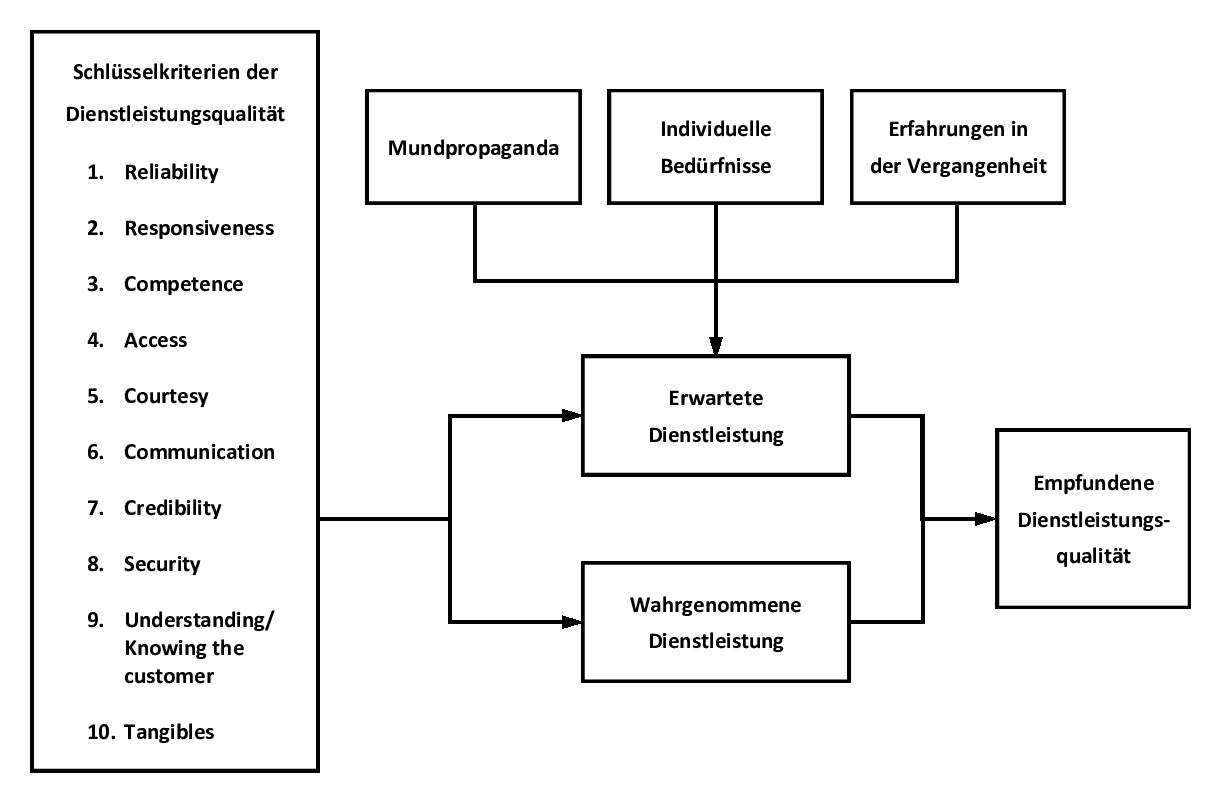
\includegraphics[width=12cm]{B2B/Bilder/determinants2}
\caption[Konsumentensicht der Dienstleistungsqualität]{Dienstleistungsqualität aus Sicht des Kunden. Die von ihm wahrgenommene Dienstleistungsqualität ist das Ergebnis aus dem Vergleich zwischen der von ihm erwarteten und der tatsächlich erhaltenen Leistung.\protect\footnotemark}
\label{determinants}
\end{figure}
\footnotetext{Abb. nach Zeithaml/Berry/Parasuraman, 1985, S. 48 \cite{Parasuraman_1985}}

\subsection{Gaps}
Aus der Befragung der Leistungsgeber gewannen Zeithaml, Berry und Parasuraman die wichtige Erkenntnis, dass aus Sicht des Unternehmens eine Reihe an Diskrepanzen, so genannte \glqq Gaps\grqq, zwischen der Vorstellung einer guten Dienstleistungsqualität und der tatsächlichen Dienstleistungserfüllung am Kunden existieren. Diese Differenzen zwischen Idealzustand und Realität können es Dienstleistern erschweren, Kunden eine Leistung zu liefern, die diese als hochqualitativ bezeichnen würden.
\\ \\
Wie in der Abbildung \ref{gap1985} erkennbar ist existieren aus Sicht des Anbieters folgende vier Diskrepanzen:\footnote{Aufzählung nach Kleinaltenkamp/Jacob, 2006, S. 54 \cite{Kleinaltenkamp2006}, Weislämle, o. Jg., S. 2 \cite{Weislaemle} und Crezelius, 2015, S. 1 \cite{Crezelius2015}}
\begin{itemize}
\item Gap 1 (Wahrnehmungslücke): Die Erwartungen der Kunden an eine Dienstleistung werden vom Management falsch interpretiert oder sind diesem gar nicht erst bekannt. Ursachen hierfür können eine unzulängliche Marktforschung, mangelhafte Kommunikation und ein unzureichendes Kundenmanagement sein.
\newpage
\item Gap 2 (Entwicklungslücke): Die vom Management verstandene Erwartung der Kunden an eine einwandfreie Dienstleistung werden in den Spezifikationen für die Dienstleistungserbringung falsch übersetzt oder nicht detailliert genug standardisiert. Gründe hierfür liegen in der mangelhaften Kundenorientierung oder Flexibilität und damit dem Festhalten an bestehenden Prozessen, obwohl sich die Anforderungen der Kunden verändert haben. Tritt diese Diskrepanz in Verbindung mit dem ersten Gap auf, potenzieren sich die Differenzen zwischen der Kundenerwartung und der von Mitarbeitern des Unternehmens umzusetzenden Dienstleistung.
\begin{figure} [t]
\centering
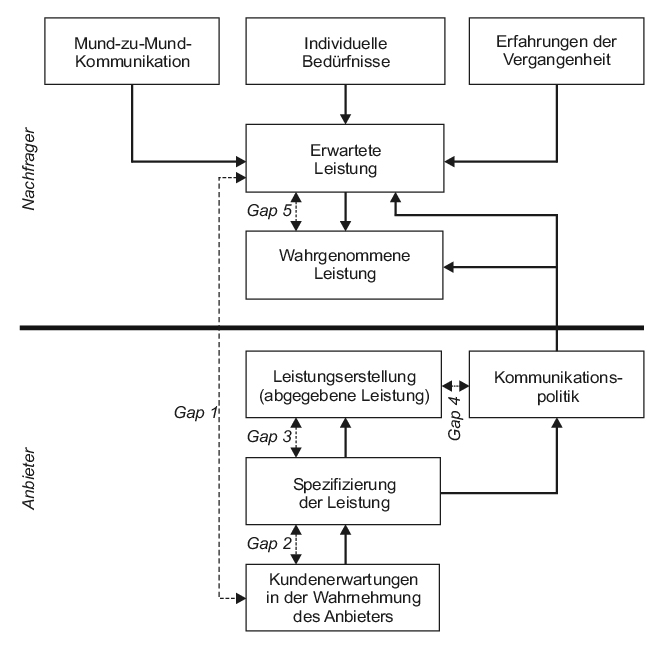
\includegraphics[width=10cm]{B2B/Bilder/gap1988}
\caption[GAP-Modell]{Das GAP-Modell nach Zeithaml, Berry und Parasuraman. Der obere Teil zeigt die Dienstleistungsqualität aus Sicht der Kunden, der untere Teil aus Sicht des Unternehmens. \protect\footnotemark}
\label{gap1985}
\end{figure}
\footnotetext{Abb. aus Kleinaltenkamp/Jacob, 2006, S. 55 \cite{Kleinaltenkamp2006} nach Zeitham/Berry/Parasuraman, 1988, S. 36 \cite{Zeithaml_1988}}
\item Gap 3 (Leistungslücke): Wird die spezifizierte Dienstleistung, zum Beispiel auf Grund von Defiziten im Prozess- und Personalmanagement, in der Realität nicht so erbracht, wie sie vom Management definiert worden ist, kann es zu einer weiteren Abweichungen von den Vorstellungen der Kunden kommen. Weiterhin kann auch die unzureichende Integration des Kunden in den Prozess der Dienstleistungserbringung diese Diskrepanz vergrößern.
\item Gap 4 (Kommunikationslücke): Die vom Unternehmen nach außen kommunizierten Informationen über die möglichen Dienstleistungen stimmen nicht mit den tatsächlich vom Unternehmen erbrachten Dienstleistungen überein. Diese Kommunikationslücke entsteht beispielsweise auf Grund einer unausgereiften Marketingkommunikation. Im Gegensatz zu den anderen Diskrepanzen wirkt sich diese nicht nur auf die vom Unternehmen erbrachte Dienstleistung aus, sondern auch auf die vom Kunden erwartete Dienstleistung. In der Folge werden die dem Kunden versprochenen Leistungen nicht oder nur unzureichend erbracht, was zu Enttäuschung bei eben jenen führt.
\end{itemize}
\noindent Die fünfte Diskrepanz, die so genannte Kundenlücke, ergibt sich schließlich aus der Summe und dem Zusammenwirken der aufgezählten Gaps 1-4. Je nach Ausprägung der ersten vier Diskrepanzen weicht eine vom Unternehmen erbrachte Dienstleistung mehr oder weniger stark von den Erwartungen der Kunden ab. Wird die Erwartungshaltung nicht erfüllt, führt dies zu Unzufriedenheit bei den Konsumenten und somit zu einer negativ wahrgenommenen Dienstleistungsqualität. Diese Sicht des Kunden auf die Dienstleistungsqualität wurde bereits in Unterabschnitt \ref{dienstleistungsqualitaet} näher erläutert.
\\ \\
Ein Unternehmen sollte daher stets darum bemüht sein, seine Prozesse dahingehend zu optimieren, diese Lücken zu minimieren, um seinen Kunden die bestmögliche Dienstleistungserfahrung bieten zu können.
\section{Kundenintegration}
\label{kundenintegration}
Die Charakteristika von bestimmten Dienstleistungen machen eine direkte Beteiligung des Kunden unabdingbar. Durch die immer stärker werdende Modularisierung und damit Individualisierbarkeit von Dienstleistungsangeboten, kann es von Vorteil sein, den Kunden durch eine Zusammenarbeit in die Prozesse, die zur Erbringung der Dienstleistung führen (\glqq uno-actu\grqq -Prinzip), oder in die zu erbringende Dienstleistung selbst zu integrieren.\footnote{vgl. Fähnrich, 2009, S. 4 \cite{Faehnrich2009}}  Dadurch werden die Kunden Teil des Erstellungsprozesses, können sich währenddessen selbst verwirklichen sowie Fehler sofort wahrnehmen und korrigieren. Zusätzlich wird den Kunden dadurch ein Gefühl der Kontrolle, Sicherheit und Wertschätzung vermittelt.\footnote{vgl. Fähnrich, 2009, S. 11 \cite{Faehnrich2009}} Durch Kundenintegration in die Dienstleistungsprozesse sind passendere auf die Kunden und deren Bedürfnisse zugeschnittene Services umsetzbar, was zu einer gesteigerten Servicequalität und Kundenzufriedenheit führt.


\chapter{GAP-Modell und Kundenintegration}
\label{kapitel3}
Wie bereits in Abschnitt \ref{kundenintegration} erläutert, ist eine Mitwirkung von Kunden vor allem dann von Nöten, wenn diesen eine individualisierte Dienstleistung oder ein spezifisch auf seine Anforderungen zugeschnittenes Produkt geliefert werden soll. In vielen Branchen ist dies Standard und liegt in der Natur der jeweiligen Geschäftsbereiche, wie zum Beispiel im Anlagengeschäft. Hier ist die individuelle Angebotsgestaltung auf Grund der Unterschiedlichkeit der einzelnen Bedarfsfälle oftmals ein Kernstück im Kundengeschäft. Aber auch im Bereich der Produktentwicklung spielt eine Individualisierung eine immer größere Rolle. Die Produktindividualisierung stellt dabei im Gegensatz zu einer strengen Einhaltung und festgesetzten Standards oder möglichst schneller Innovationserrungenschaften eine eigenständige Wettbewerbsstrategie dar.\footnote{vgl. Kleinaltenkamp, 2006, S. 50 \cite{Kleinaltenkamp2006}}
\\ \\
Um einen Leistungserstellungsprozess auf die Bedürfnisse des Kunden hin ausrichten zu können, ist ein Mindestmaß an Kundenbeteiligung erforderlich. Mit der Kenntnis seiner individuellen Anforderungen und Bedürfnisse ist es möglich, die Spezifikationen für einen individuellen Erstellungsprozess festzulegen. Im Falle einer derartigen Kundenintegration wird diese selbst ein wichtiger Teil des Leistungserstellungsprozesses. Abbildung \ref{produktentwicklung} zeigt beispielhaft einen entsprechenden Produktentwicklungsprozess von der Ideenfindung bis zur Markteinführung mit den jeweiligen Schnittstellen einer erfolgten Kundenintegration.
\begin{figure} [H]
\centering
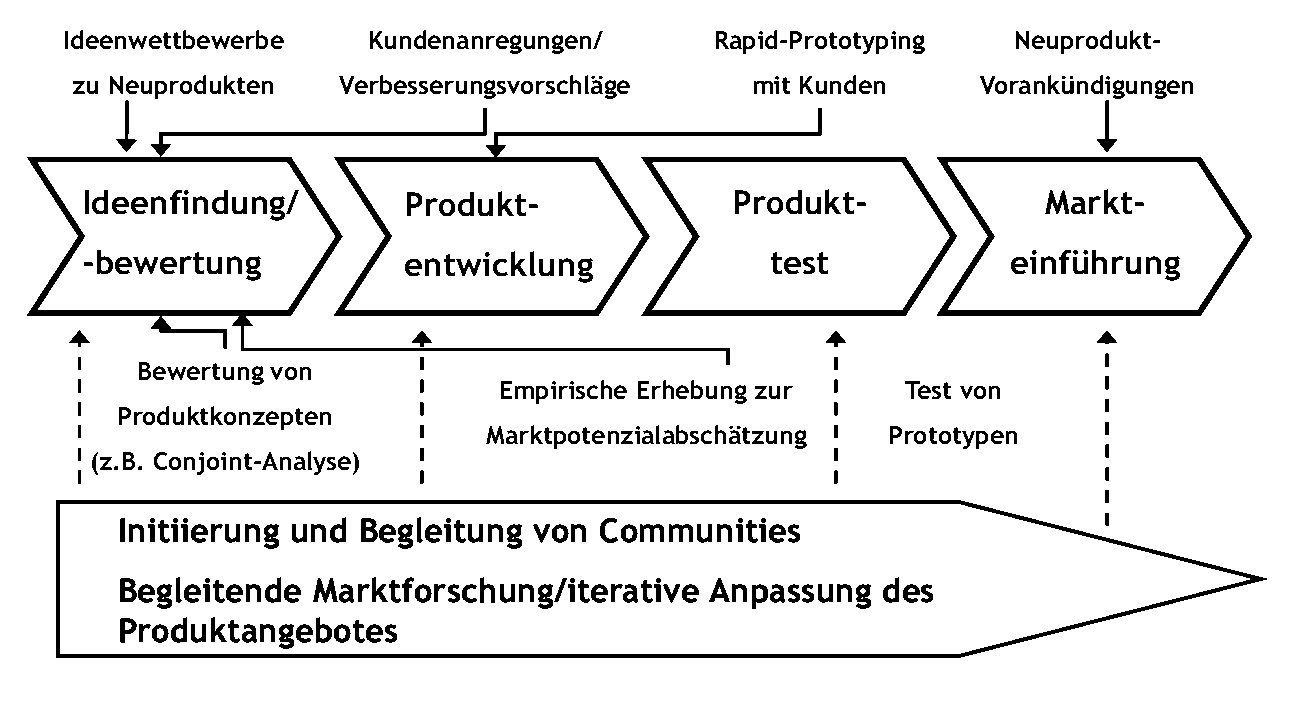
\includegraphics[width=12cm]{B2B/Bilder/produktentwicklung}
\caption[Produktentwicklungsprozess]{Beispiel eines Produktentwicklungsprozess mit verschiedenen Möglichkeiten der Kundenintegration. \protect\footnotemark}
\label{produktentwicklung}
\end{figure}
\footnotetext{Abb. aus Löbel, 2016, S. 21 \cite{Loebel2016} nach Backhaus/Voeth, 2014, S. 229 \cite{Backhaus2014}}
\newpage
\noindent Damit die vom Kunden zur Verfügung gestellten Informationen zur Spezifikation des Leistungserstellungsprozesses korrekt interpretiert und umgesetzt werden, empfiehlt sich hier ebenfalls die Anwendung des GAP-Modells. Auch die Individualisierung eines Produktes ist im Kern eine Dienstleistung, die den Kunden erbracht wird. Somit besitzt der Kunde ähnlich wie im Dienstleistungssektor gewisse Erwartungen an die Leistungen eines Unternehmens, die sich aus der Mundpropaganda, den eigenen Bedürfnissen und den bisherigen Erfahrungen speisen. Die Aufgabe des Unternehmens ist es nun, die vom Kunden mitgeteilten Anforderungen und Bedürfnisse an das zu individualisierende Produkt richtig zu verstehen (Gap 1 - Wahrnehmungslücke), diese interpretierten Vorstellungen in für den Leistungsentwicklungsprozess kompatible Spezifikationen zu überführen (Gap 2 - Entwicklungslücke) und anschließend korrekt umzusetzen (Gap 3 - Leistungslücke), damit das vom Unternehmen gelieferte Produkt dem vom Kunden erwarteten Produkt bestmöglich entspricht (Gap 5 - Kundenlücke). Weiterhin ist es ausschlaggebend, dass das Unternehmen seine möglichen Produkte und Angebote, im Speziellen die Art und der Umfang des potenziellen Einflusses auf den Leistungsentwicklungsprozess, den Kunden korrekt kommuniziert, das dies ansonsten zu falschen Erwartungen auf der Kundenseite führen würde (Gap 4 - Kommunikationslücke).
\\ \\
Mit Hilfe der Anwendung des GAP-Modells im Rahmen der Kundenintegration in Leistungserstellungsprozesse sind Unternehmen in der Lage, in der Kommunikation und in der Absprache mit Kunden ganz natürlich auftretende Diskrepanzen zu minimieren.



\chapter{Zusammenfassung und Fazit}
In dieser Hausarbeit wurde im Kapitel \ref{kapitel1} zunächst auf das Thema \glqq Das GAP-Modell im Kontext der Kundenintegration\grqq{}einführend hingearbeitet. Weiterhin wurden die möglichen Probleme bei Mensch-zu-Mensch-Kommunikation erörtert. Im nachfolgenden Kapitel \ref{kapitel2} wurden die Grundlagen für ein besseres Verständnis der Hintergründe des GAP-Modells sowie der Kundenintegration vermittelt. Im letzten Kapitel \ref{kapitel3} wurde erläutert, welche Bedeutung die Anwendung des GAP-Modells im Kontext der Kundenintegration zukommt.
\\ \\
Zusammenfassend lässt sich sagen, dass sich GAP-Modell auch im Kontext der Kundenintegration anwenden lässt. Es ist ein unverzichtbares Hilfsmittel für Unternehmen, ihre Leistungserstellungsprozesse so zu gestalten, dass die möglichen Diskrepanzen beim Informationsfluss mit Kunden möglichst gering ausfallen oder ganz ausbleiben. Dadurch steigt die Effektivität des Leistungserstellungsprozesses und die jeweiligen Kunden erhalten die tatsächlich von ihnen gewünschte beziehungsweise benötigte Leistung.
\\ \\
Es gilt als Folge der Kundenintegration jedoch zu beachten, dass diese die Effizienz eines Unternehmens stark beeinträchtigen können. Um letztendlich dennoch von den positiven Effekten der Kundenintegration profitieren zu können, sollten Unternehmen entsprechende Controlling-Maßnahmen durchführen.\footnote{vgl. Kleinaltenkamp, 2006, S. 54 f. \cite{Kleinaltenkamp2006}}
